%-----------------------------------LICENSE------------------------------------%
%   This file is part of Mathematics-and-Physics.                              %
%                                                                              %
%   Mathematics-and-Physics is free software: you can redistribute it and/or   %
%   modify it it under the terms of the GNU General Public License as          %
%   published by the Free Software Foundation, either version 3 of the         %
%   License, or (at your option) any later version.                            %
%                                                                              %
%   Mathematics-and-Physics is distributed in the hope that it will be useful, %
%   but WITHOUT ANY WARRANTY; without even the implied warranty of             %
%   MERCHANTABILITY or FITNESS FOR A PARTICULAR PURPOSE.  See the              %
%   GNU General Public License for more details.                               %
%                                                                              %
%   You should have received a copy of the GNU General Public License along    %
%   with Mathematics-and-Physics.  If not, see <https://www.gnu.org/licenses/>.%
%------------------------------------------------------------------------------%

%   Use the standalone class for displaying the tikz image on a small PDF.
\documentclass[crop,tikz]{standalone}

%   Import the tikz package and use the arrows.meta library for the LaTeX arrow.
\usepackage{tikz}
\usetikzlibrary{arrows.meta}

%   Begin the document.
\begin{document}

    %   Draw the figure.
    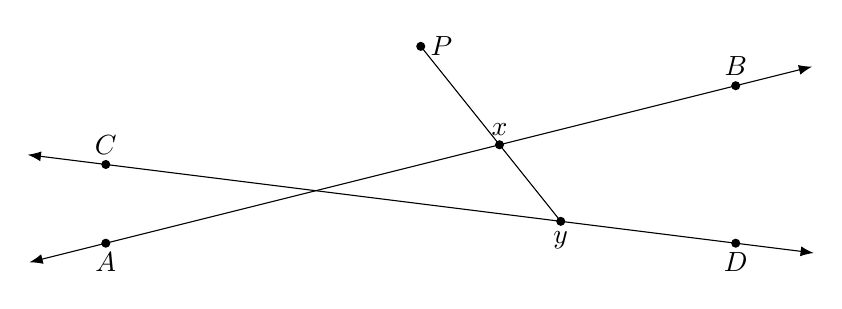
\begin{tikzpicture}[>=Latex]

        %   Label all of the points in the drawing.
        \coordinate (A) at (-4.0000, -1.0000);
        \coordinate (B) at ( 4.0000,  1.0000);
        \coordinate (C) at (-4.0000,  0.0000);
        \coordinate (D) at ( 4.0000, -1.0000);
        \coordinate (P) at ( 0.0000,  1.5000);
        \coordinate (x) at ( 1.0000,  0.2500);
        \coordinate (y) at ( 1.7778, -0.7222);

        %   Draw the two lines.
        \draw[<->, shorten >=-1cm, shorten <=-1cm] (A) to (B);
        \draw[<->, shorten >=-1cm, shorten <=-1cm] (C) to (D);

        %   Draw the perspective line of rP onto y.
        \draw (P) to (y);

        %   Draw dots at all of the vertices.
        \draw[fill=black] (P) circle (0.5mm);
        \draw[fill=black] (A) circle (0.5mm);
        \draw[fill=black] (B) circle (0.5mm);
        \draw[fill=black] (C) circle (0.5mm);
        \draw[fill=black] (D) circle (0.5mm);
        \draw[fill=black] (x) circle (0.5mm);
        \draw[fill=black] (y) circle (0.5mm);

        %   Label all of the vertices.
        \node at (A) [below] {$A$};
        \node at (B) [above] {$B$};
        \node at (C) [above] {$C$};
        \node at (D) [below] {$D$};
        \node at (P) [right] {$P$};
        \node at (x) [above] {$x$};
        \node at (y) [below] {$y$};
    \end{tikzpicture}
\end{document}
